\documentclass[en]{university}

\faculty{Department of Computer Engineering}
\course{Computer Networks}
\subject{Homework 3}
\professor{Dr. Jafari}
\student{Parsa Mohammadian}

\begin{document}

\setupdocument

\section{}
Software-Defined Networking or SDN is a networking architecture that uses software-based controllers or APIs\footnote{Application Programming Interface} to implement network functions for hardware-based infrastructure. 

The architecture of SDN is shown in Figure \ref{fig:sdn}. Since the control layer of network is decoupled from the infrastructure layer, SDN has the following criterias:
\begin{itemize}
    \item 
\end{itemize}

\begin{figure}
    \centering
    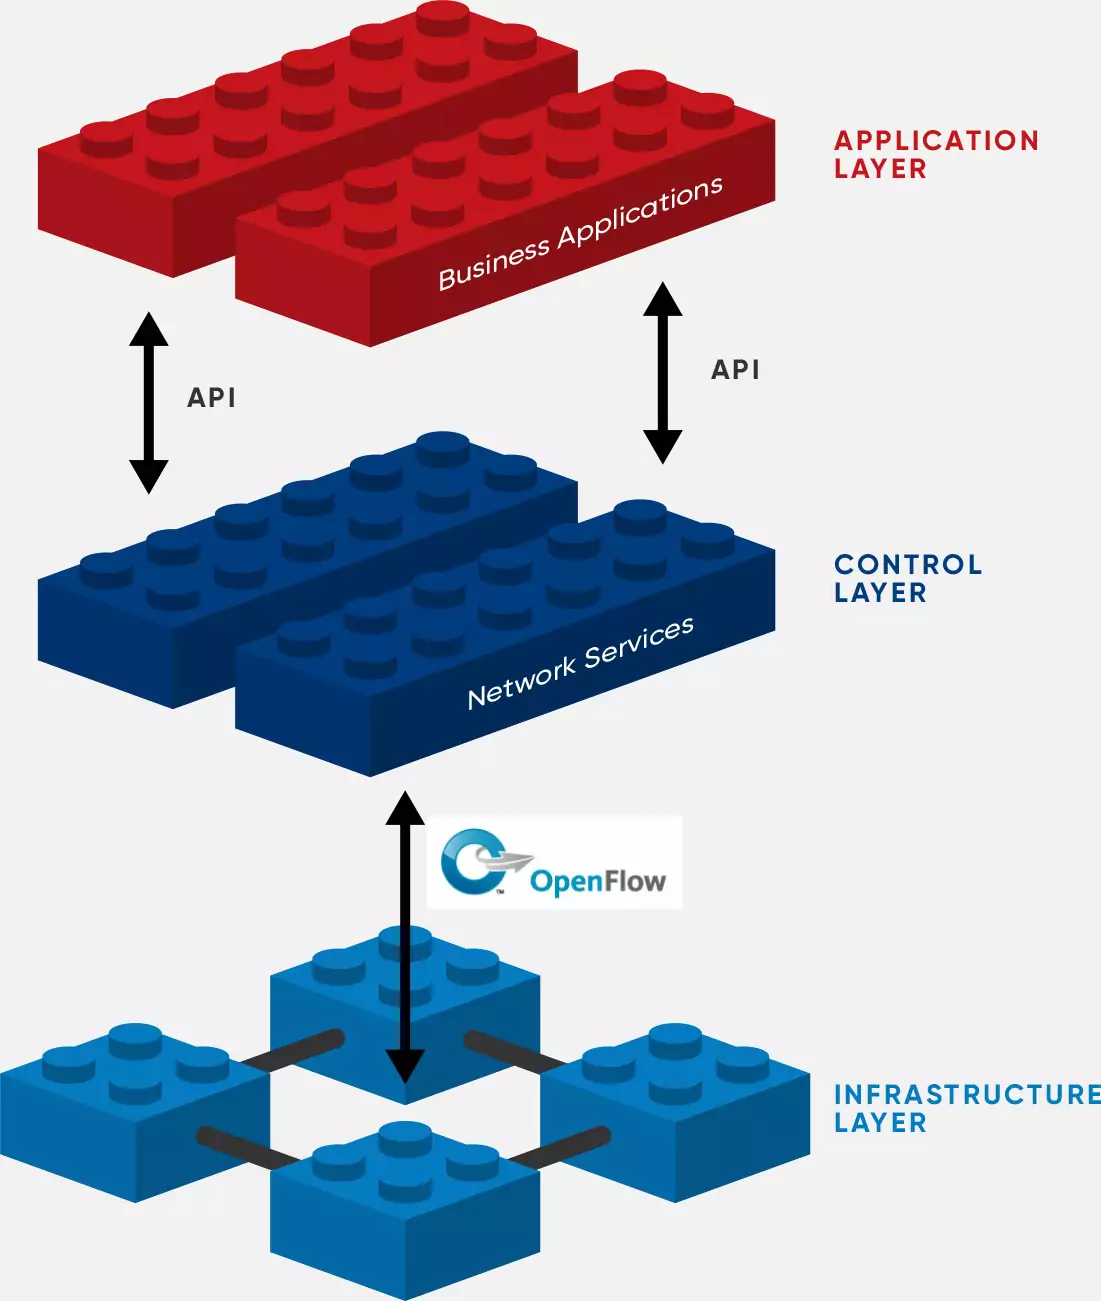
\includegraphics[width=0.8\textwidth]{resources/sdn-architecture-img.png}
    \caption{SDN Architecture}
    \label{fig:sdn}
\end{figure}


\subsubsection*{Resources}
\begin{itemize}
    \item \href{https://youtube.com/watch?v=Z5Gi2Bpd82M}{\url{https://youtube.com/watch?v=Z5Gi2Bpd82M}}
    \item \href{https://youtube.com/watch?v=Nh2hXUuKXyQ}{\url{https://youtube.com/watch?v=Nh2hXUuKXyQ}}
    \item \href{https://opennetworking.org/sdn-definition/}{\url{https://opennetworking.org/sdn-definition/}}
\end{itemize}

\section{}
\subsection{}

\subsection{}

\section{}
\subsection{}

\subsection{}

\section{}
\subsection{}

\subsection{}

\section{}

\end{document}